\chapter{Hardware}\label{ch:hardware}
The hardware part of the project consisted of initially three separate parts, a drawing contraptions, a battery holder, and a bluetooth shield. 
In the final version of the robot we ended up not using the battery holder due to problems with the manufacturing hardware. 
In this chapter we will first present the chassis modification, before moving on to present the circuitry needed for the bluetooth module. 

\section{Chassis modifications}
The problem we initially underestimated was how we should make the physical robot draw on paper. While a front or back mounted pen would be an easy solution this would not create the angles properly, and thus was not a real viable options. The clearence below the robot was to small for anything to fit underneath it, and the battery was placed in such a way that nothing could fit between the wheels of the robot (see figure~\ref{fig:robotUnder}). In order to fix this problem we designed a batteryholder which could be mounted on top of the robot (see figure~\ref{fig:batteryHolder}), but due to techinical problems witht the 3D printes we were not able to test this design. And we had to resort to an alternative solution using velcro to position the battery at the back of the robot and duct tape to add a counterweight at the front of the robot to provide stability (see figures in~\ref{fig:robot}). 

\bigskip\noindent
While this solved the problem of making room beneath the robot we still had multiple issues with getting the robot to draw properly. These issues were mainly due to inaccuracies in the 3D-printing environment meaning the the spring used to push the drawing tip into the paper would get snagged inside its container (figures~\ref{fig:pencilHolder} and~\ref{fig:pencilHolderReal}).


\begin{figure}[H]
	\centering
	\subfloat[Battery holder\label{fig:batteryHolder}]{
		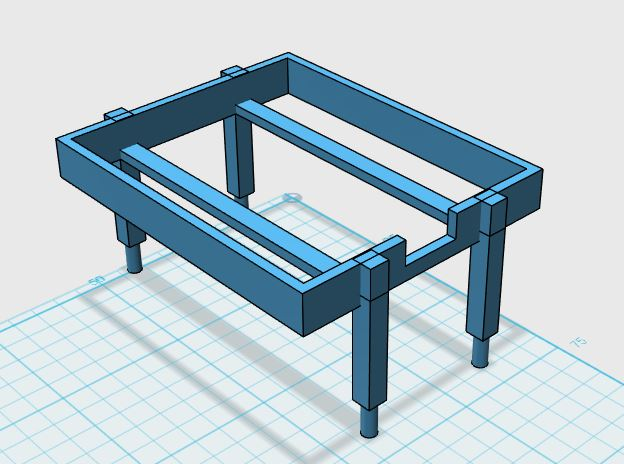
\includegraphics[width=0.4\linewidth]{images/BatteryHolder.JPG}
	}
	\subfloat[Pencil holder\label{fig:pencilHolder}]{
		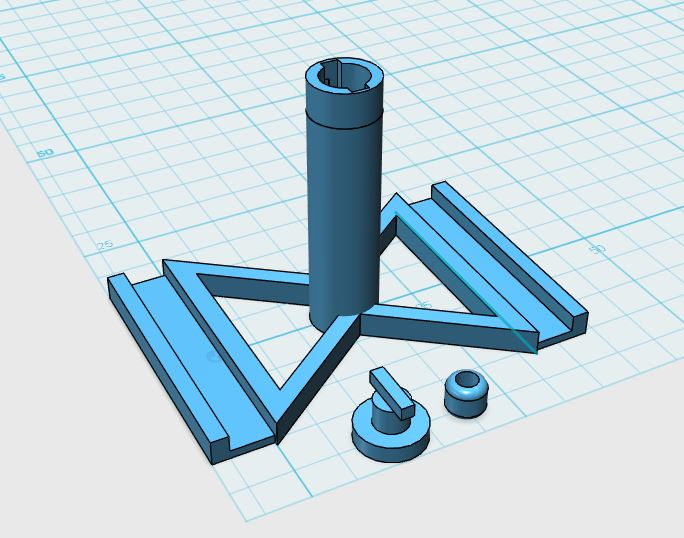
\includegraphics[width=0.4\linewidth]{images/PencilHolder.JPG}
	}\\
	\subfloat[Printed pencil holder\label{fig:pencilHolderReal}]{
		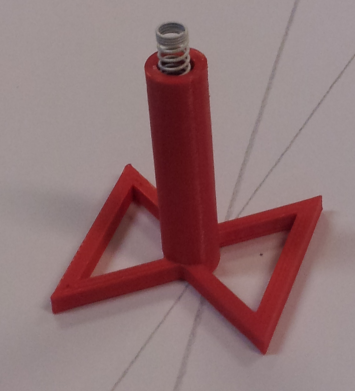
\includegraphics[width=0.4\linewidth]{images/penHolder.png}
	}
	\caption{3D printed utilities}
	\label{fig:3d}
\end{figure}
\begin{figure}[H]
	\centering
	\subfloat[Front of robot\label{fig:robotFront}]{
		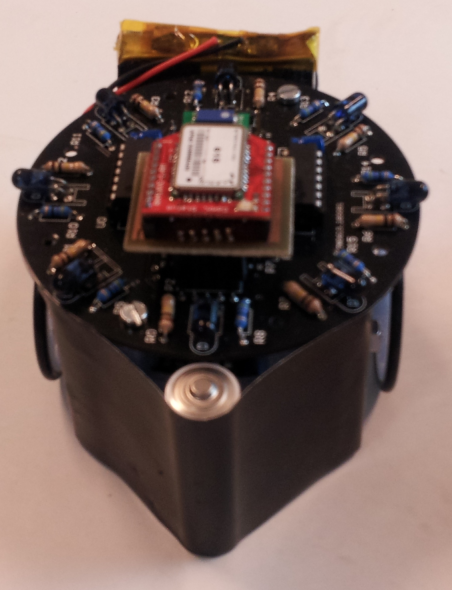
\includegraphics[width=0.4\linewidth]{images/robotFront.png}
	}
	\subfloat[Back of robot\label{fig:robotBack}]{
		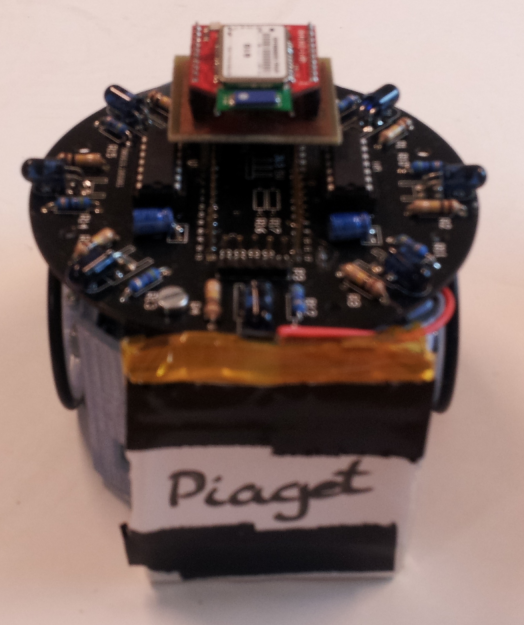
\includegraphics[width=0.4\linewidth]{images/robotBack.png}
	}\\
	\subfloat[Underside of robot\label{fig:robotUnder}]{
		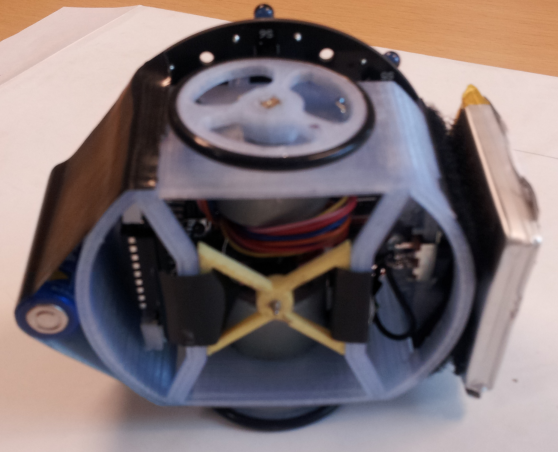
\includegraphics[width=0.4\linewidth]{images/robotUnder.png}
	}
	\subfloat[Robot drawing an angle\label{fig:robotDrawing}]{
		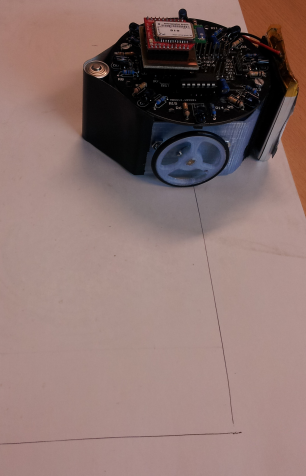
\includegraphics[width=0.4\linewidth]{images/robotDrawing.png}
	}
	\caption{Pictures of the robot}
	\label{fig:robot}
\end{figure}

\section{Bluetooth circuit board}
The \chirp team had previously tested using bluetooth communication between an android device and the robot. We therefore got help in creating the inital circuitry for our bluetooth module(figure~\ref{fig:circuitDrawing}). This drawing was at this point designed in the Eagle software in order to make it possible to produce at a later stage(~\ref{fig:circuitDesign}). 

\bigskip\noindent
The basic functionality of the circuit is to create a mapping between the receiver (\textbf{RX}) and transmission (\textbf{TX}) signals on the arduino and bluetooth module. In addition to the data signals the circuit board needed to map a 3.3V power supply (\textbf{VDD}) and a ground connection (\textbf{GND}) to the bluetooth module (see schematic in figure~\ref{fig:bluetoothSchematic}).

\image{images/schematicBluetooth2.PNG}{\linewidth}{Schematic of the bluetooth shield. Components on the right is the bluetooth module.}{fig:bluetoothSchematic}

\bigskip\noindent
As seen in figure~\ref{fig:bluetoothSchematic} we used a two components between the arduino TX signal and the bluetooth module RX (a 220$\Omega$ resistor and 3.3V zener diode). This was because the arduino operates on 5V, while the bluetooth module expected only 3.3V. Mapping these directly would most likely result in the destruction of the module. It should here be noted that the schematic does in show a normal diode, but the circuit is design for a zener diode and using a normal diode would not work.

\bigskip\noindent
It can be seen in figure~\ref{fig:circuitProto} that some soldering around the board was necessary on the prototype. The prototype did however lead us to conclude that the circuit itself was functional and we were able to proceed with creating all the circuit boards that we needed. 
Figure~\ref{fig:circuitTrans} shows the template used in the etching process when creating these boards. While figure~\ref{fig:circuitboard} shows the circuit board alongside with the bluetooth module we used for our robots. The complete assembly of the robot can be seen in figure~\ref{fig:robotDrawing}.

\begin{figure}[!htb]
	\centering
	\subfloat[Inital circuit\label{fig:circuitDrawing}]{
		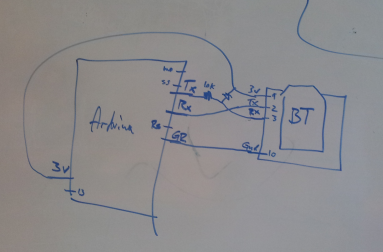
\includegraphics[width=0.4\linewidth]{images/bluetoothCircuit.png}
	}
	\subfloat[Created in circuit designer\label{fig:circuitDesign}]{
		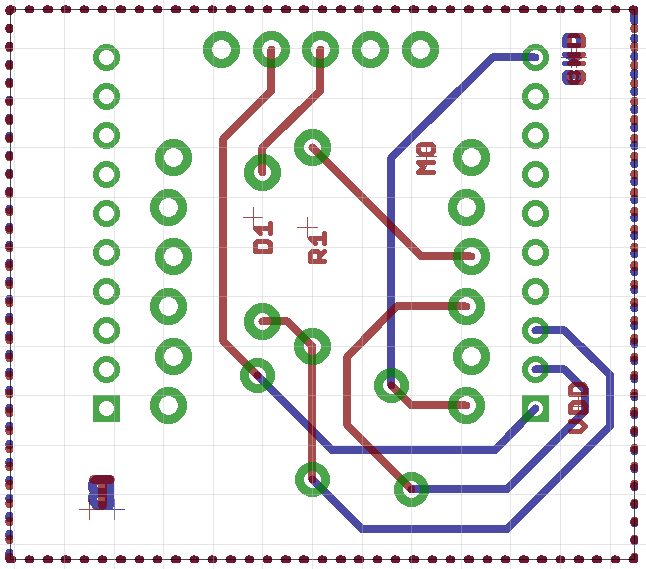
\includegraphics[width=0.4\linewidth]{images/circuitDrawing.PNG}
	}\\
	\subfloat[Prototype template\label{fig:circuitProtoTrans}]{
		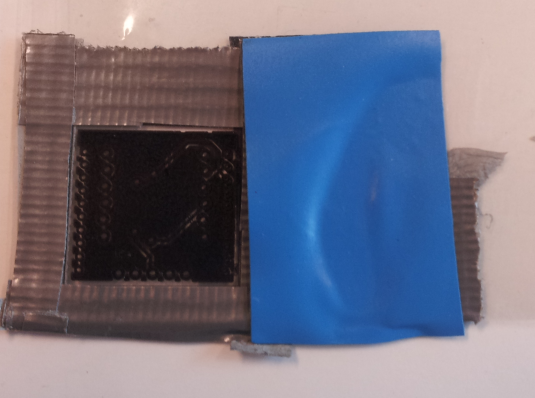
\includegraphics[width=0.4\linewidth]{images/bluetoothProtoTrans.png}
	}
	\subfloat[Prototype circuitboard\label{fig:circuitProto}]{
		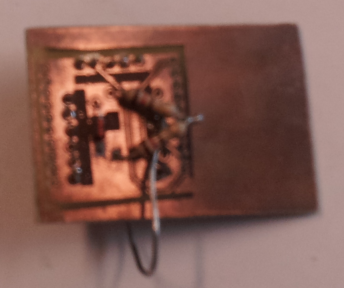
\includegraphics[width=0.4\linewidth]{images/bluetoothProto.png}
	}\\
	\subfloat[Finished template\label{fig:circuitTrans}]{
		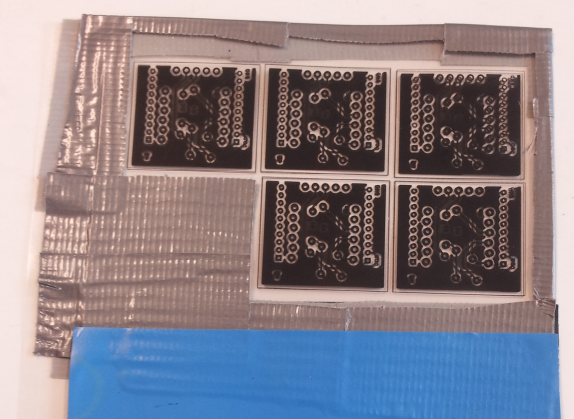
\includegraphics[width=0.4\linewidth]{images/bluetoothTrans.png}
	}
	\subfloat[Finished circuitboard\label{fig:circuitboard}]{
		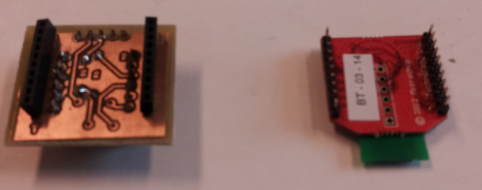
\includegraphics[width=0.4\linewidth]{images/bluetooth.png}
	}
	\caption{Circuit boards}
	\label{fig:circuit}
\end{figure}
